\chapter{Neutrinos}

In 1930 Wolfgang Pauli postulates a particle, that he calls neutron, to explain how beta decay could conserve energy, momentum, and angular momentum. 
This new particle would have to be neutral and non-interacting. 
Describing his idea as a "desperate remedy'', even Pauli was unsure if this particle would ever be detected. 
In 1933 Enrico Fermi further develops the theory of beta decay in which Pauli's particle plays an integral part. 
It becomes clear that this particle, which Fermi renames the neutrino ("little neutral one''),
 must be very light, less than 1\% the mass of the proton, and interact very weakly with matter.
The discovery of this neutrino wouldn't happen until 20 years later.


\section{Discovery of the Neutrino}



\section{Neutrinos in the Standard Model} 

\section{Lepton Mixing}

\section{Neutrino Oscillation}

\section{Discovery of Neutrino Oscillation}


%\begin {table}[!htbp]
%\end{table}


%begin{figure}[!htbp]
%\center
%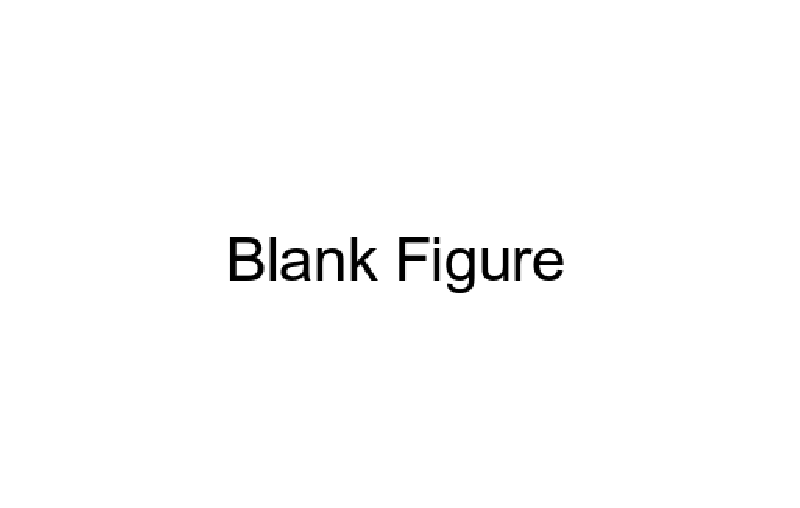
\includegraphics[width = 0.5\columnwidth]{tex/2-neutrinos-images/blank.eps}
%\caption{Figure in a subfolder.} 
%\label{fig:test2}
%\end{figure}


Testing citing \cite{Huber}.
